\begin{figure}[H]
    \centering
    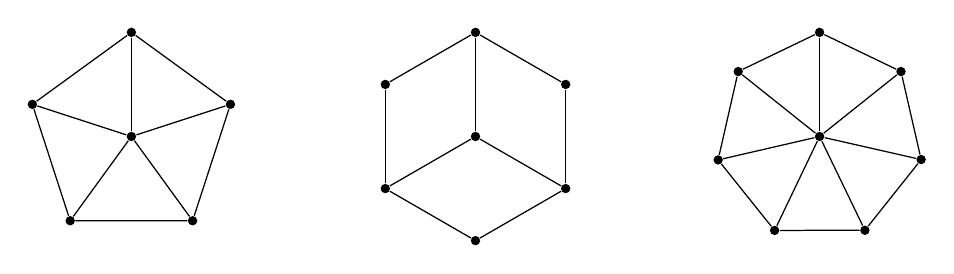
\begin{tikzpicture}[
        scale=1.15,
        vertex/.style={circle, fill=black, inner sep=1.2pt},
        edge/.style={line width=0.45pt}
    ]
    
    % Left graph
    \begin{scope}[xshift=0cm]
        \foreach \i/\ang in {1/90,2/18,3/-54,4/-126,5/162}
            \node[vertex] (a\i) at (\ang:1.15) {};
        \node[vertex] (ac) at (0,0) {};
    
        \foreach \i/\j in {1/2,2/3,3/4,4/5,5/1}
            \draw[edge] (a\i) -- (a\j);
        \foreach \i in {1,2,3,4,5}
            \draw[edge] (ac) -- (a\i);
    \end{scope}
    
    % Middle graph
    \begin{scope}[xshift=3.8cm]
        \foreach \i/\ang in {1/90,2/30,3/-30,4/-90,5/-150,6/150}
            \node[vertex] (b\i) at (\ang:1.15) {};
        \node[vertex] (bc) at (0,0) {};
    
        \foreach \i/\j in {1/2,2/3,3/4,4/5,5/6,6/1}
            \draw[edge] (b\i) -- (b\j);
        \foreach \i in {1,3,5}
            \draw[edge] (bc) -- (b\i);
    \end{scope}
    
    % Right graph
    \begin{scope}[xshift=7.6cm]
        \foreach \i/\ang in {1/90,2/38.6,3/-12.8,4/-64.2,5/-115.6,6/-167,7/141.4}
            \node[vertex] (c\i) at (\ang:1.15) {};
        \node[vertex] (cc) at (0,0) {};
    
        \foreach \i/\j in {1/2,2/3,3/4,4/5,5/6,6/7,7/1}
            \draw[edge] (c\i) -- (c\j);
        \foreach \i in {1,2,3,4,5,6,7}
            \draw[edge] (cc) -- (c\i);
    \end{scope}
    
    \end{tikzpicture}
    \caption{Forbidden vertex minors of circle grpahs.}
    \end{figure}